\ctexset{%%% do not add blank rows
 chapter/format+=\raggedright, % +adding \raggedright left align for chapter
}
\chapter{绪论}
\addentoc{chapter}{Introduction} % 中文章标题为“引言”,英文目录条目为“Introduction”
\setcounter{page}{1}
\pagenumbering{arabic}

\setlength{\parskip}{0pt}	% 行距为0
\setstretch{1.25} % 设置1.25倍行距


\section{研究背景与意义}
\addentoc{section}{Research Background and Significance} 


\subsection{图/参考文献}
\addentoc{subsection}{Figure}


单个参考文献\cite{2024_刘巍_Article}。

多个参考文献\cite{2024_刘巍_Article,2023_刘巍_Article,2019_刘巍_Article}。



图参考。
可见参见\autoref{fig:TestPic}。
\begin{figure}[!htb]
	\centering
	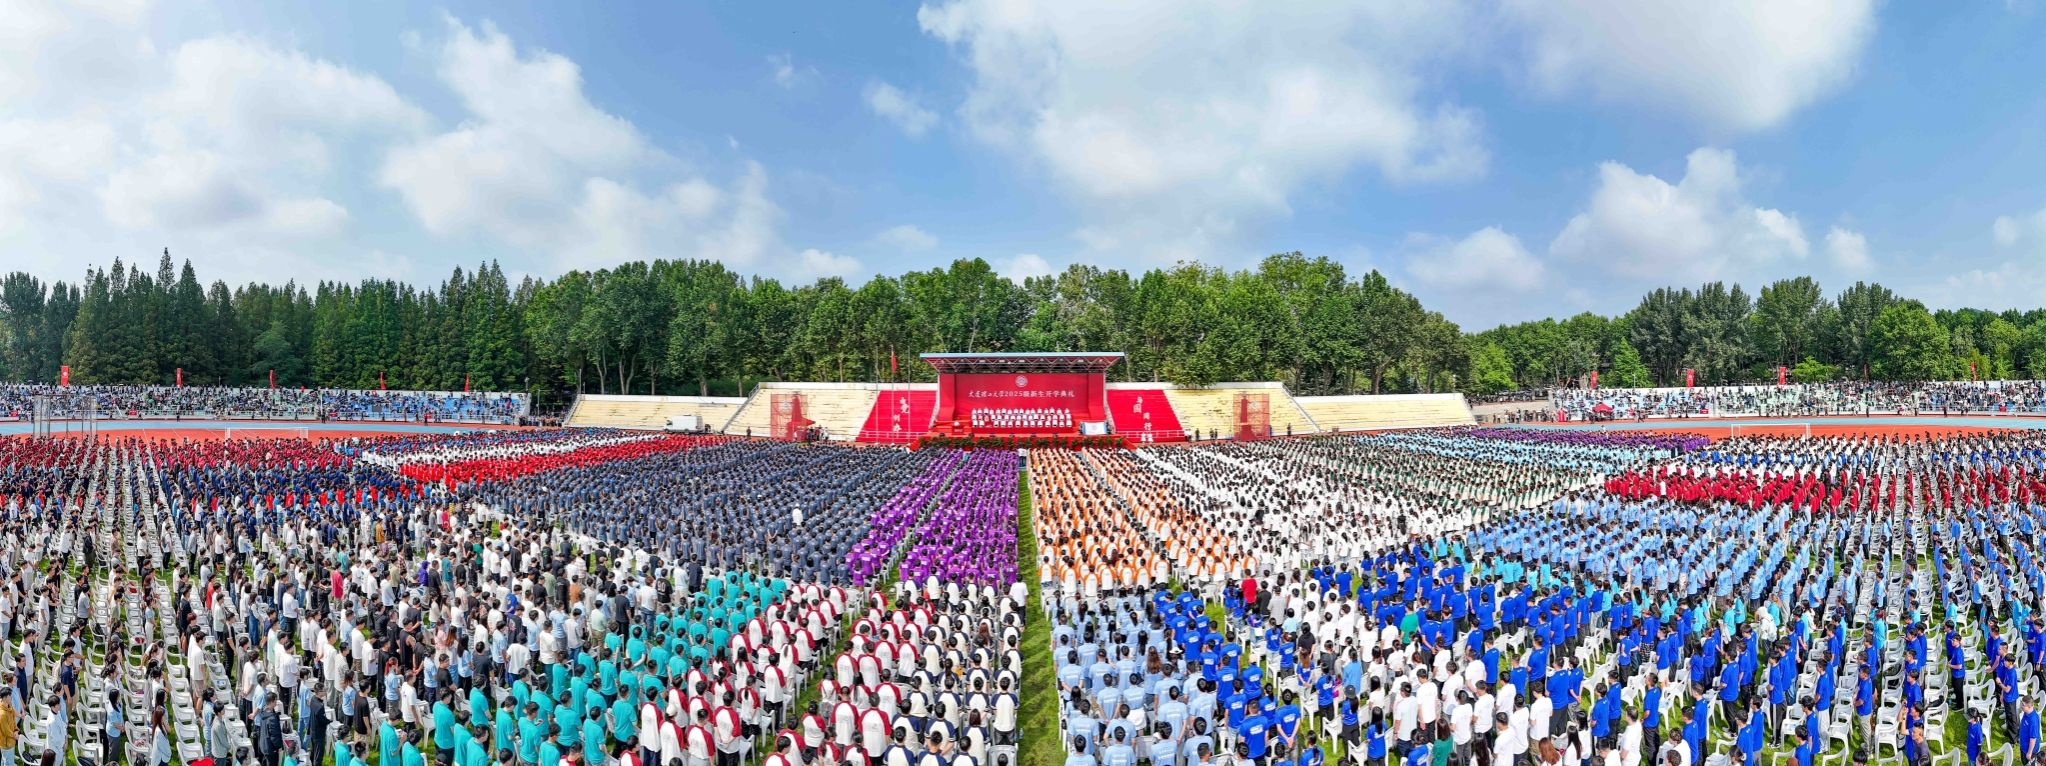
\includegraphics[width=0.9\textwidth]{figures/ch1/TestPic.jpg}
	\bicaption{大连理工大学开学典礼}{Opening Ceremony of Year 2025 at DUT}
	\label{fig:TestPic}
\end{figure}



表参考。
可见参见\autoref{tab:tableTest}。

\begin{table}[!htb]
	\centering
	\bicaption{表格示例}{Illustration of a table}
	\label{tab:tableTest}
	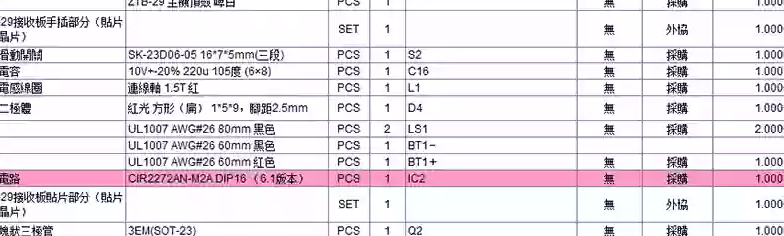
\includegraphics[width=0.9\textwidth]{figures/ch1/tableTest.png}
\end{table}